\documentclass[11pt]{article}
  \usepackage{pgfplots}
  \usepackage{graphicx}
  \pgfplotsset{compat=1.5.1} % 用来保证双 y 轴时两个 y 轴的 label 正确显示

  %%%%%%%%%%%%%%%%%%%%%%%%%%%%%%%%%%%%%%%%%
% Lachaise Assignment
% Structure Specification File
% Version 1.0 (26/6/2018)
%
% This template originates from:
% http://www.LaTeXTemplates.com
%
% Authors:
% Marion Lachaise & François Févotte
% Vel (vel@LaTeXTemplates.com)
%
% License:
% CC BY-NC-SA 3.0 (http://creativecommons.org/licenses/by-nc-sa/3.0/)
% 
%%%%%%%%%%%%%%%%%%%%%%%%%%%%%%%%%%%%%%%%%

%----------------------------------------------------------------------------------------
%	PACKAGES AND OTHER DOCUMENT CONFIGURATIONS
%----------------------------------------------------------------------------------------

\usepackage{amsmath,amsfonts,stmaryrd,amssymb} % Math packages

\usepackage{enumerate} % Custom item numbers for enumerations

\usepackage[ruled]{algorithm2e} % Algorithms

\usepackage[framemethod=tikz]{mdframed} % Allows defining custom boxed/framed environments

\definecolor{codegreen}{rgb}{0,0.2,0}
\definecolor{codegray}{rgb}{0.5,0.5,0.5}
\definecolor{codepurple}{rgb}{0.5,0.2,0.5}
\definecolor{codekeyword}{rgb}{0.5,0,0.22}

\usepackage{listings} % File listings, with syntax highlighting
\lstset{
	commentstyle=\color{codegreen},
	keywordstyle=\color{codekeyword},
	numberstyle=\tiny\color{codegray},
	stringstyle=\color{codepurple},
	basicstyle=\footnotesize,
	basicstyle=\ttfamily, % Typeset listings in monospace font
}

%----------------------------------------------------------------------------------------
%	DOCUMENT MARGINS
%----------------------------------------------------------------------------------------

\usepackage{geometry} % Required for adjusting page dimensions and margins

\geometry{
	paper=a4paper, % Paper size, change to letterpaper for US letter size
	top=2.5cm, % Top margin
	bottom=3cm, % Bottom margin
	left=2.5cm, % Left margin
	right=2.5cm, % Right margin
	headheight=14pt, % Header height
	footskip=1.5cm, % Space from the bottom margin to the baseline of the footer
	headsep=1.2cm, % Space from the top margin to the baseline of the header
	% showframe, % Uncomment to show how the type block is set on the page
}

%----------------------------------------------------------------------------------------
%	FONTS
%----------------------------------------------------------------------------------------

\usepackage[utf8]{inputenc} % Required for inputting international characters
\usepackage[T1]{fontenc} % Output font encoding for international characters

% \usepackage{XCharter} % Use the XCharter fonts\usepackage{XCharter} % Use the XCharter fonts

%----------------------------------------------------------------------------------------
%	COMMAND LINE ENVIRONMENT
%----------------------------------------------------------------------------------------

% Usage:
% \begin{commandline}
%	\begin{verbatim}
%		$ ls
%		
%		Applications	Desktop	...
%	\end{verbatim}
% \end{commandline}

\mdfdefinestyle{commandline}{
	innertopmargin=\baselineskip,
	leftmargin=0pt,
	rightmargin=0pt,
	innerleftmargin=5pt,
	middlelinecolor=black!50!white,
	middlelinewidth=2pt,
	frametitlerule=false,
	backgroundcolor=black!5!white,
	frametitle={Command Line},
	frametitlefont={\normalfont\sffamily\color{white}\hspace{-1em}},
	frametitlebackgroundcolor=black!50!white,
	nobreak,
	font=\small
}

% Define a custom environment for command-line snapshots
\newenvironment{commandline}{
	\medskip
	\begin{mdframed}[style=commandline]
}{
	\end{mdframed}
	\medskip
}

%----------------------------------------------------------------------------------------
%	FILE CONTENTS ENVIRONMENT
%----------------------------------------------------------------------------------------

% Usage:
% \begin{file}[optional filename, defaults to "File"]
%	File contents, for example, with a listings environment
% \end{file}

\mdfdefinestyle{file}{
	innertopmargin=\baselineskip,
	innerbottommargin=0.8\baselineskip,
	topline=false, bottomline=false,
	leftline=false, rightline=false,
	leftmargin=0cm,
	rightmargin=0cm,
	singleextra={%
		\draw[fill=black!10!white](P)++(0,-1.2em)rectangle(P-|O);
		\node[anchor=north west]
		at(P-|O){\ttfamily\mdfilename};
		%
		\def\l{3em}
		\draw(O-|P)++(-\l,0)--++(\l,\l)--(P)--(P-|O)--(O)--cycle;
		\draw(O-|P)++(-\l,0)--++(0,\l)--++(\l,0);
	},
	nobreak,
	font=\small
}

% Define a custom environment for file contents
\newenvironment{file}[1][File]{ % Set the default filename to "File"
	\medskip
	\newcommand{\mdfilename}{#1}
	\begin{mdframed}[style=file]
}{
	\end{mdframed}
	\medskip
}

%----------------------------------------------------------------------------------------
%	NUMBERED QUESTIONS ENVIRONMENT
%----------------------------------------------------------------------------------------

% Usage:
% \begin{question}[optional title]
%	Question contents
% \end{question}

\mdfdefinestyle{question}{
	innertopmargin=1.2\baselineskip,
	innerbottommargin=0.8\baselineskip,
	roundcorner=5pt,
	nobreak,
	singleextra={%
		\draw(P-|O)node[xshift=1em,anchor=west,fill=white,draw,rounded corners=5pt]{%
		Question \theQuestion\questionTitle};
	},
}

\newcounter{Question} % Stores the current question number that gets iterated with each new question

% Define a custom environment for numbered questions
\newenvironment{question}[1][\unskip]{
	\bigskip
	\stepcounter{Question}
	\newcommand{\questionTitle}{~#1}
	\begin{mdframed}[style=question]
}{
	\end{mdframed}
	\medskip
}

%----------------------------------------------------------------------------------------
%	WARNING TEXT ENVIRONMENT
%----------------------------------------------------------------------------------------

% Usage:
% \begin{warn}[optional title, defaults to "Warning:"]
%	Contents
% \end{warn}

\mdfdefinestyle{warning}{
	topline=false, bottomline=false,
	leftline=false, rightline=false,
	nobreak,
	singleextra={%
		\draw(P-|O)++(-0.5em,0)node(tmp1){};
		\draw(P-|O)++(0.5em,0)node(tmp2){};
		\fill[black,rotate around={45:(P-|O)}](tmp1)rectangle(tmp2);
		\node at(P-|O){\color{white}\scriptsize\bf !};
		\draw[very thick](P-|O)++(0,-1em)--(O);%--(O-|P);
	}
}

% Define a custom environment for warning text
\newenvironment{warn}[1][Warning:]{ % Set the default warning to "Warning:"
	\medskip
	\begin{mdframed}[style=warning]
		\noindent{\textbf{#1}}
}{
	\end{mdframed}
}

%----------------------------------------------------------------------------------------
%	INFORMATION ENVIRONMENT
%----------------------------------------------------------------------------------------

% Usage:
% \begin{info}[optional title, defaults to "Info:"]
% 	contents
% 	\end{info}

\mdfdefinestyle{info}{%
	topline=false, bottomline=false,
	leftline=false, rightline=false,
	nobreak,
	singleextra={%
		\fill[black](P-|O)circle[radius=0.4em];
		\node at(P-|O){\color{white}\scriptsize\bf i};
		\draw[very thick](P-|O)++(0,-0.8em)--(O);%--(O-|P);
	}
}

% Define a custom environment for information
\newenvironment{info}[1][Info:]{ % Set the default title to "Info:"
	\medskip
	\begin{mdframed}[style=info]
		\noindent{\textbf{#1}}
}{
	\end{mdframed}
}

\usepackage{fontspec}
\usepackage{indentfirst}
\usepackage{booktabs}
\usepackage{graphicx}
\usepackage{subfigure}
\usepackage{url}
\usepackage{flushend, cuted}
\usepackage{color}
\usepackage{enumitem} 

\XeTeXlinebreaklocale "zh"
\XeTeXlinebreakskip = 0pt plus 1pt
\setlength{\parindent}{2em} % 2em 代表首行缩进两个字符
% \linespread{1.2} % 设置行间距

\usepackage{tikz}
\usetikzlibrary{graphs, positioning, quotes, shapes.geometric} % Include the file specifying the document structure and custom commands

  % 如果提示没有字体,请修改此处的字体路径为当前编译文件的相对路径
  \setmainfont[ExternalLocation=../.template/]{STZHONGS.ttf}

  % 用于在代码内显示中文
  \usepackage{xeCJK}
  \setCJKmonofont[ExternalLocation=../.template/]{STZHONGS.ttf}

  \usepackage[font=small,labelfont=bf,tableposition=top]{caption}

  \DeclareCaptionLabelFormat{andtable}{#1~#2  \&  \tablename~\thetable}
  
  %----------------------------------------------------------------------------------------
  %	ASSIGNMENT INFORMATION
  %----------------------------------------------------------------------------------------
  
  \title{\Large 数据库原理及应用课程作业 \#2 \\
  \LARGE 思政资源数据库创建与数据管理操作} % Title of the assignment
  
  \author{杨睿妮 \texttt{(2018011205014)} \\ \url{yangruinii@foxmail.com}} % Author name and email address
  
  \date{电子科技大学 --- \today} % University, school and/or department name(s) and a date
  
  %----------------------------------------------------------------------------------------
  
  \begin{document}
  
  \maketitle % Print the title

  \section{实验说明}
  \begin{itemize}
    \item 采用 SQL定义数据库模式以及操作数据和控制数据、采用数据操作语言 DML 对预备的思政素材进行增删改查、采用数据控制语言 DCL 进行安全权限许可控制
    \item 完成树状学科目录的前端展示
  \end{itemize}

  \section{实验原理}
  SQL的工作机理见图\ref{tab:SQL1}
    \begin{figure*}[h]
    \centering
    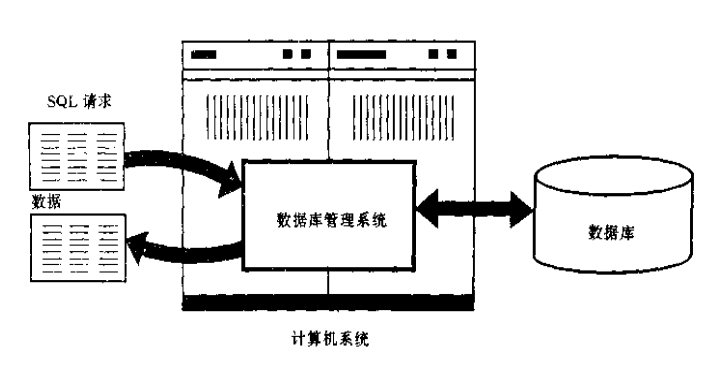
\includegraphics[width=0.7\textwidth]{SQL工作机理.png}
    \caption{SQL工作机理}
    \label{tab:SQL1}
  \end{figure*}

  SQL的工作过程见图\ref{tab:SQL2}
    \begin{figure*}[h]
    \centering
    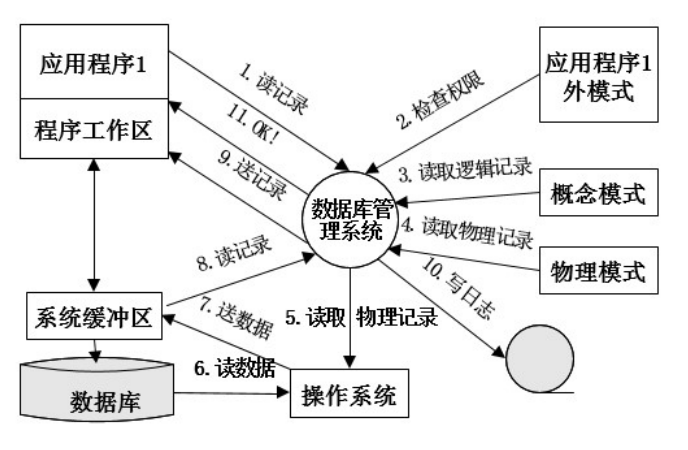
\includegraphics[width=0.7\textwidth]{SQL工作过程.png}
    \caption{SQL工作过程}
    \label{tab:SQL2}
  \end{figure*}

  \section{实验环境}
  实验环境如表 \ref{tab:env} 所示。
  \begin{table}[h]
    \centering
    \caption{实验环境}
    \label{tab:env}
    \begin{tabular}{ll}
      \hline
      处理器 & lntel(R) Core(TM) i5-8300H CPU @2.30GHz \\
      \hline
      内存 & 16GB \\
      \hline
      软件 & Sybase PowerDesigner Version 16.5; SQL Server 2012\\
      \hline
      操作系统 & Windows 10 \\
      \hline
      语言 & Python 3.8.5; HTML; JaveScript; CSS\\
      \hline
      框架 & Flask 1.1.2 \\
      \hline
      
    \end{tabular}
  \end{table}

  \section{实验步骤}
  \subsection{利用 Power Designer 的自动模式创建功能构建思政资源数据库}

  利用 Power Designer 的自动模式生成了\verb|lab_1.sql|脚本,将其导入SQL Server中,结果见图\ref{fig:powerdesignerResult},具体的SQL语句见附录\ref{apd:labsql}。
  \begin{figure*}[h]
    \centering
    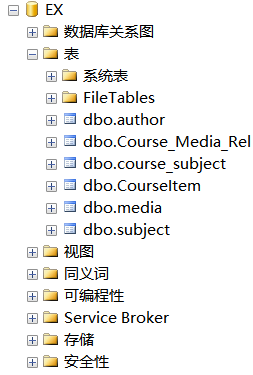
\includegraphics[width=0.4\textwidth]{PDResult.png}
    \caption{数据库创建结果}
    \label{fig:powerdesignerResult}
  \end{figure*}

  \subsection{采用 SQL 定义各个实体模式上的实体完整性、参照完整性和自定义完整性}
  在实验一建立数据库中时,已经对相关的属性进行了约束:满足关系的主码不能取空值;参照关系中每个元素的外码要么为空,要么等于被参照关系中某个元素的主码;对关系中每个属性的取值的限制做了具体定义。在后续的数据增删查改中也满足了三种完整性。

  \subsection{采用 SQL 语句创建视图,为思政资源素材检索提供外模式(用户模式)}
  在本次实验中,建立了名为 \verb|View_Course_Type| 的视图,功能为选择出\verb|type = '1'| 的思政素材,单独组成一个视图,提供外模式。使用的语句见\verb|create-view.sql|。
  \begin{file}[create-view.sql]
    \begin{lstlisting}[language=sql]
      create view View_Course_Type
      as
         select * from dbo.CourseItem where type = '1'
      go
      
      select * from View_Course_Type
    \end{lstlisting}
  \end{file}

  \subsection{采用 SQL 在实体模式上创建单属性索引,在视图上建立复合索引}
  为了提升思政资源素材的检索效率,在\verb|dbo.CourseItem|上为\verb|keyword|建立名为\verb|CourseKeyword|的索引,提高用户根据关键词查找素材的效率,具体语句见\verb|create-index.sql|,结果见\ref{fig:index1}。
  \begin{file}[create-index.sql]
    \begin{lstlisting}[language=sql]
      CREATE INDEX CourseKeyword
      ON dbo.CourseItem (keyword)
    \end{lstlisting}
  \end{file}

  \begin{figure*}[h]
    \centering
    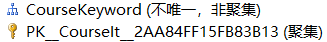
\includegraphics[width=0.6\textwidth]{index1.png}
    \caption{CourseKeyword索引}
    \label{fig:index1}
  \end{figure*}

  为了提升思政资源素材在混合属性上的检索效率,我们利用\verb|WITH SCHEMABINDING|关键字建立新的视图,以便于后续在该视图上建立复合索引。\verb|WITH SCHEMABINDING|是防止视图所引用的表在视图未被调整的情况下发生改变的选项。

  建立了名为\verb|View_For_Index|的视图,选择出表\verb|dob.CourseItem|中\verb|type|为“1”的实体。并且在该视图上,基于列\verb|author|和\verb|keyword|建立名为\verb|IDX_V1|的索引,便于用户基于作者以及关键字查找思政素材。具体语句见\verb|create-view-index.sql|,结果见\ref{fig:IDX1}。

  \begin{file}[create-view-index.sql]
    \begin{lstlisting}[language=sql]
      create view View_For_Index
      WITH SCHEMABINDING
      AS
      select courseDesc, courseID,keyword, author, source 
      from dbo.CourseItem where type = '1'
   go
   
   CREATE UNIQUE CLUSTERED INDEX IDX_V1
      ON View_For_Index(author, keyword);
   GO
    \end{lstlisting}
  \end{file}

  \begin{figure*}[h]
    \centering
    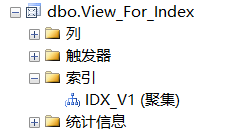
\includegraphics[width=0.4\textwidth]{IDX1.png}
    \caption{在视图上的复合索引"IDX\_V1"}
    \label{fig:IDX1}
  \end{figure*}

  \subsection{采用 Insert 语句将采编的思政资源素材录入到数据库中}
  插入采编者信息,采用的语句见\verb|insert-author.sql|,具体结果见\ref{fig:insert}。

  \begin{file}[insert-author.sql]
    \begin{lstlisting}[language=sql]
    insert into dbo.author(authorID, authorName) values(1,'Ruini Yang');
    insert into dbo.author(authorID, authorName) values(2,'Yifei Zhang');
    insert into dbo.author(authorID, authorName) values(3,'Culaccino');
    insert into dbo.author(authorID, authorName) values(4,'Komorebi');
    insert into dbo.author(authorID, authorName) values(5,'Goya');
    insert into dbo.author(authorID, authorName) values(6,'Ternura');
    insert into dbo.author(authorID, authorName) values(7,'Alkaid');
    // ...
    \end{lstlisting}
  \end{file}

  \begin{figure*}[h]
    \centering
    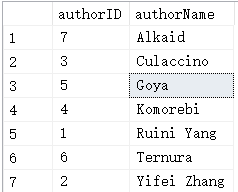
\includegraphics[width=0.4\textwidth]{insert.png}
    \caption{插入采编者}
    \label{fig:insert}
  \end{figure*}

  插入学科信息,采用的语句见\verb|insert-subject.sql|,具体结果见\ref{fig:insert-subject}。

  \begin{file}[insert-subject.sql]
    \begin{lstlisting}[language=sql]
  insert into dbo.subject(subjectID, subjectName, parentID) values
  (1,'基础学科', '0');
  insert into dbo.subject(subjectID, subjectName, parentID) values
  (2,'信息科技', '0');
  insert into dbo.subject(subjectID, subjectName, parentID) values
  (3,'医药卫生科技', '0');
  insert into dbo.subject(subjectID, subjectName, parentID) values
  (4,'哲学与人文科学', '0');
  insert into dbo.subject(subjectID, subjectName, parentID) values
  (5,'基础化学', '1');
    // ...
    \end{lstlisting}
  \end{file}

  \begin{figure*}[h]
    \centering
    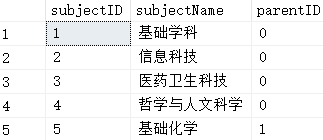
\includegraphics[width=0.5\textwidth]{insert-subject.png}
    \caption{插入学科信息}
    \label{fig:insert-subject}
  \end{figure*}

  插入思政素材,采用的语句见\verb|insert-course.sql|,具体结果见\ref{fig:insert-course}。

  \begin{file}[insert-course.sql]
    \begin{lstlisting}[language=sql]
  insert into dbo.CourseItem(courseID, authorID, courseDesc, courseName, 
  keyword, author, source, type, cnt) values(1, 8,'维护安全问题', 
  'Linux操作系统维护技术探析', 'Linux系统', '方木龙', 
  '中移互联网有限公司', '1', 0);
  insert into dbo.CourseItem(courseID, authorID, courseDesc, courseName, 
  keyword, author, source, type, cnt) values(2, 9,'非易失主存构建存储系统
  , '非易失主存的系统软件研究进展', '非易失主存', '舒继武', '中国科学 : 
  信息科学', '2', 0);
  insert into dbo.CourseItem(courseID, authorID, courseDesc, courseName, 
  keyword, author, source, type, cnt) values(3, 10,'混合教学模式', 
  '混合教学模式在“操作系统”中的研究和实践', '混合模式', '杨婷婷', 
  '无线互联科技', '1', 0);
  insert into dbo.CourseItem(courseID, authorID, courseDesc, courseName, 
  keyword, author, source, type, cnt) values(4, 11,'课程教学内容重组', 
  '基于 OBE理念的操作系统原理课程教学内容重组', '操作系统', '张秋红', 
  '兰州文理学院学报', '1', 0);
    // ...
    \end{lstlisting}
  \end{file}

  \begin{figure*}[h]
    \centering
    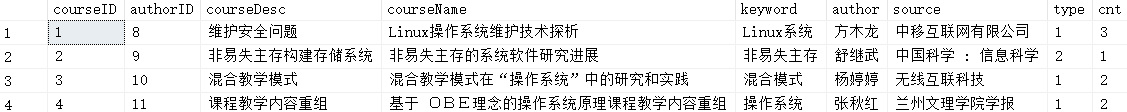
\includegraphics[width=\textwidth]{insert-course.png}
    \caption{插入思政素材}
    \label{fig:insert-course}
  \end{figure*}

  插入思政素材与学科之间的多对多关系,采用的语句见\verb|insert-rel.sql|,具体结果见可以体现在前端界面显示上,点击学科可以显示出相应的思政素材。

  \begin{file}[insert-rel.sql]
    \begin{lstlisting}[language=sql]
      insert into dbo.course_subject(courseID, subjectID) values(1, 11)
      insert into dbo.course_subject(courseID, subjectID) values(2, 11)
      insert into dbo.course_subject(courseID, subjectID) values(3, 11)
      insert into dbo.course_subject(courseID, subjectID) values(4, 11)
    // ...
    \end{lstlisting}
  \end{file}

  插入多媒体素材素材,采用的语句见\verb|insert-media.sql|,具体结果见\ref{fig:insert-media}。

  \begin{file}[insert-media.sql]
    \begin{lstlisting}[language=sql]
      insert into dbo.media(mediaID, authorID,mediaName,url) values(1,2,
      '王道考研-操作系统','https://www.bilibili.com/video/BV1YE411D7nHfrom
      =search
    &seid=13181938279769288528')
      insert into dbo.media(mediaID, authorID,mediaName,url) values(2,2,
      '谭浩强老师C语言教程程序设计','https://www.bilibili.com/video/
      BV1VW41187zq?from=search&seid=12389279456804192620')
      insert into dbo.media(mediaID, authorID,mediaName,url) values(3,1,
      '计算机软件技术基础','https://www.bilibili.com/video/BV1xa4y1j7ZN?
      from=search&seid=1409768092267906681')
    // ...
    \end{lstlisting}
  \end{file}

  \begin{figure*}[h]
    \centering
    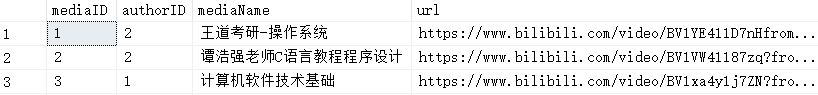
\includegraphics[width=0.9\textwidth]{insert-media.png}
    \caption{插入多媒体素材}
    \label{fig:insert-media}
  \end{figure*}



  \subsection{采用 Update 语句更新思政资源素材的点击阅读次数}
  以将每个\verb|type|为"1"的思政素材点击次数加1为例,具体语句见\verb|update-cnt.sql|,结果见图\ref{fig:update}。

  \begin{file}[update-cnt.sql]
    \begin{lstlisting}[language=sql]
      update dbo.CourseItem set cnt = cnt + 1
      where type = '1'
    \end{lstlisting}
  \end{file}

  \begin{figure*}[h]
    \centering
    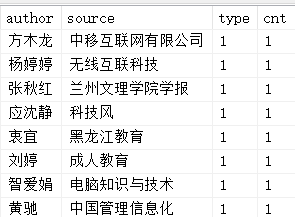
\includegraphics[width=0.4\textwidth]{update.png}
    \caption{更新操作}
    \label{fig:update}
  \end{figure*}

  \subsection{采用 Select 语句实现思政资源素材的关键词模糊检索}
  以对关键词中含有“系统”进行模糊检索为例,具体语句见\verb|select.sql|,结果见图\ref{fig:select}。

  \begin{file}[select.sql]
    \begin{lstlisting}[language=sql]
      select * from dbo.CourseItem 
      where keyword like '%系统%'
    \end{lstlisting}
  \end{file}

  \begin{figure*}[h]
    \centering
    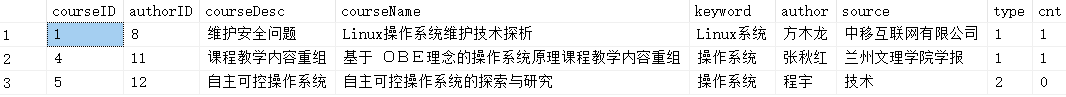
\includegraphics[width=\textwidth]{select.png}
    \caption{检索操作}
    \label{fig:select}
  \end{figure*}

  \subsection{采用 Select 语句实现思政资源素材的分类别、分目录按点击阅读次数降序统计}
  以将一级目录(即没有上级学科,\verb|parentID = 0|)中,且\verb|type = 1|的学科按点击阅读次数降序统计。具体语句见\verb|desc.sql|,结果见图\ref{fig:desc}。

  \begin{file}[desc.sql]
    \begin{lstlisting}[language=sql]
      select subject.parentID, cnt,CourseItem.courseName 
      from dbo.subject,dbo.CourseItem, dbo.course_subject
      where CourseItem.courseID = course_subject.courseID 
      and subject.parentID = 0
      group by subject.parentID, cnt, CourseItem.courseName
      order by cnt desc
    \end{lstlisting}
  \end{file}

  \begin{figure*}[h]
    \centering
    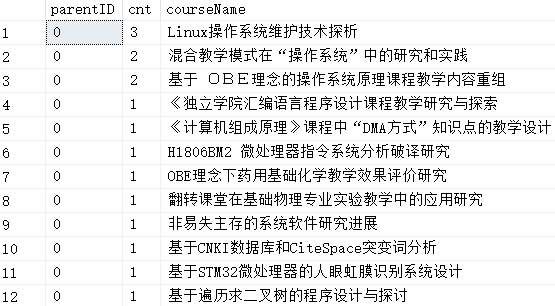
\includegraphics[width=0.7\textwidth]{desc.png}
    \caption{降序统计}
    \label{fig:desc}
  \end{figure*}

  \subsection{采用 Grant 语句为一组用户授予不同的增删改查权限许可}
  创建三个登录账号以及对应的数据库用户,具体语句见\verb|create-login.sql|。
  \begin{file}[create-login.sql]
    \begin{lstlisting}[language=sql]
    create login dba1 with password = '123', default_database = EX
    create user Wang for login dba1 with default_schema = dbo
    create login dba2 with password = '123', default_database = EX
    create user Li for login dba2 with default_schema = dbo
    create login dba3 with password = '123', default_database = EX
    create user Zhang for login dba3 with default_schema = dbo
    \end{lstlisting}
  \end{file}

  赋予三个用户不同的权限,具体语句见\verb|grant.sql|。
  \begin{file}[grant.sql]
    \begin{lstlisting}[language=sql]
      grant select on CourseItem to Wang
      grant insert on author to Li
      grant update(author, type) on CourseItem to Zhang
    \end{lstlisting}
  \end{file}

  登录\verb|dba1|账号,输入\lstinline{select * from dbo.}语句,在\verb|EX|数据库中只会出现\verb|CourseItem|的提示,与我们之前设置的权限相符合。见图\ref{fig:dba1}。

  \begin{figure*}[h]
    \centering
    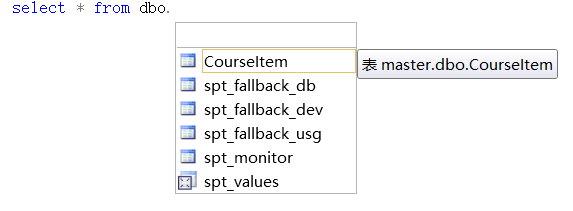
\includegraphics[width=0.7\textwidth]{dba1.png}
    \caption{dba1权限}
    \label{fig:dba1}
  \end{figure*}

  登录\verb|dba2|账号,输入\lstinline{select * from dbo.author}语句,会报错。这是由于\verb|dba2|对于表\verb|author|只有\verb|insert|权限而没有\verb|select|的权限。结果见图\ref{fig:dba2}。
  \begin{figure*}[h]
    \centering
    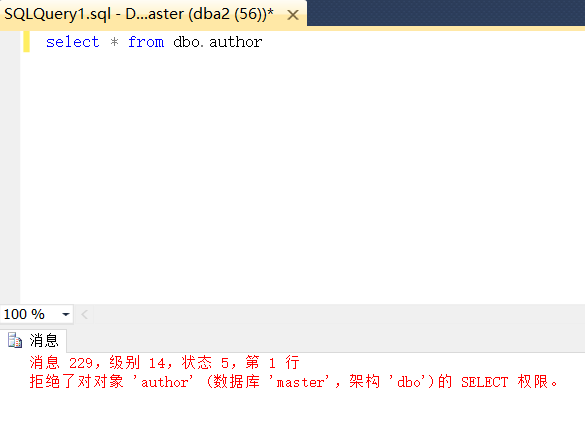
\includegraphics[width=0.7\textwidth]{dba2.png}
    \caption{dba2权限}
    \label{fig:dba2}
  \end{figure*}

  登录\verb|dba3|账号,输入\lstinline{update dbo.CourseItem set type = '2' where author = '方木龙'}语句,但是会报错“拒绝了对对象 'CourseItem' (数据库 'master',架构 'dbo')的 SELECT 权限。”通过\verb|sa|用户对\verb|dba3|用户用语句\lstinline{grant select on dbo.CourseItem to Zhang}赋予\verb|select|权限,再次执行该指令不再报错。
  
  \section{Flask框架实现数据库操作}

  本次实验后端对数据库的操作采用了\verb|Flask|框架中调用\verb|pyodbc|库对数据库数据进行调取与操作。

  以\lstinline|@app.route('/user/get/<int:id>')|路由为例,实现了在表\verb|author|中的\verb|select|操作。具体代码如下:

  \begin{file}[app.py]
    \begin{lstlisting}[language=Python]
      // ...
      @app.route('/user/get/<int:id>')
      def get(id):
          cursor = cnxn.cursor()
          cursor.execute("SELECT * from author where authorID = %d" %(id))
          result=cursor.fetchone() 
          cnxn.commit() 
          return {
              "authorID": result[0],
              "authorName": result[1]
          }
      // ...
    \end{lstlisting}
  \end{file}

  在前端发送请求结果见图\ref{fig:userget}。
  \begin{figure*}[h]
    \centering
    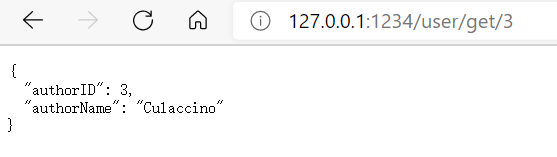
\includegraphics[width=0.7\textwidth]{userget.png}
    \caption{在author表中检索id为3的采编者并且返回name}
    \label{fig:userget}
  \end{figure*}

  以\lstinline|@app.route('/user/add', methods=['GET', 'POST'])|路由为例,实现了在表\verb|author|中添加操作。终端采用命令和具体代码如下,结果见图\ref{fig:useradd}。

  \begin{commandline}
    \begin{verbatim}
$  curl -d '{"name": "Karina", "ID": 40}' -H 'Content-Type:application/json' http://localhost:1234/user/add
    \end{verbatim}
  \end{commandline}

  \begin{file}[app.py]
    \begin{lstlisting}[language=Python]
      @app.route('/user/add', methods=['GET', 'POST'])
      def add():
          if request.method == 'POST':
              data = request.get_json()
              cursor = cnxn.cursor()
              name = data['name']
              ID = data['ID']
              cursor.execute("insert into author(authorID, authorName) 
              values(%d, '%s')" % (ID, name))
              cursor.execute("SELECT * from author")
              result=cursor.fetchall()
              cnxn.commit()
              for row in result:
                  print(row)
              return {
                  "ok": "true"
              }
    \end{lstlisting}
  \end{file}

  \begin{figure*}[h]
    \centering
    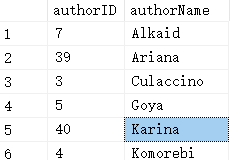
\includegraphics[width=0.4\textwidth]{useradd.png}
    \caption{在author表中添加采编者成功}
    \label{fig:useradd}
  \end{figure*}


  
  \section{前端网页展示}
  为了完成在前端展示学科的树状模型,以及点击相关学科可以展示出与该学科对应的思政素材,在\verb|app.py|中,设置了\lstinline{@app.route("/subsubject/side-item-name-<int:id>")}路由完成各级科学目录之下的学科获取,以完成网页侧边栏的树状课程目录展示;设置了\verb|@app.route("/course/<int:id>")|路由完成了对应学科下的思政素材的获取功能,并且结合JavaScript代码将其展示在网页上。以下是网页的展示,具体的前端代码\verb|index.js|;\verb|styles.css|;\verb|index.html|,以及后端\verb|Flask|代码\verb|app.py|代码详见附录。

  网页的主页见图\ref{fig:home}。
  \begin{figure*}[h]
    \centering
    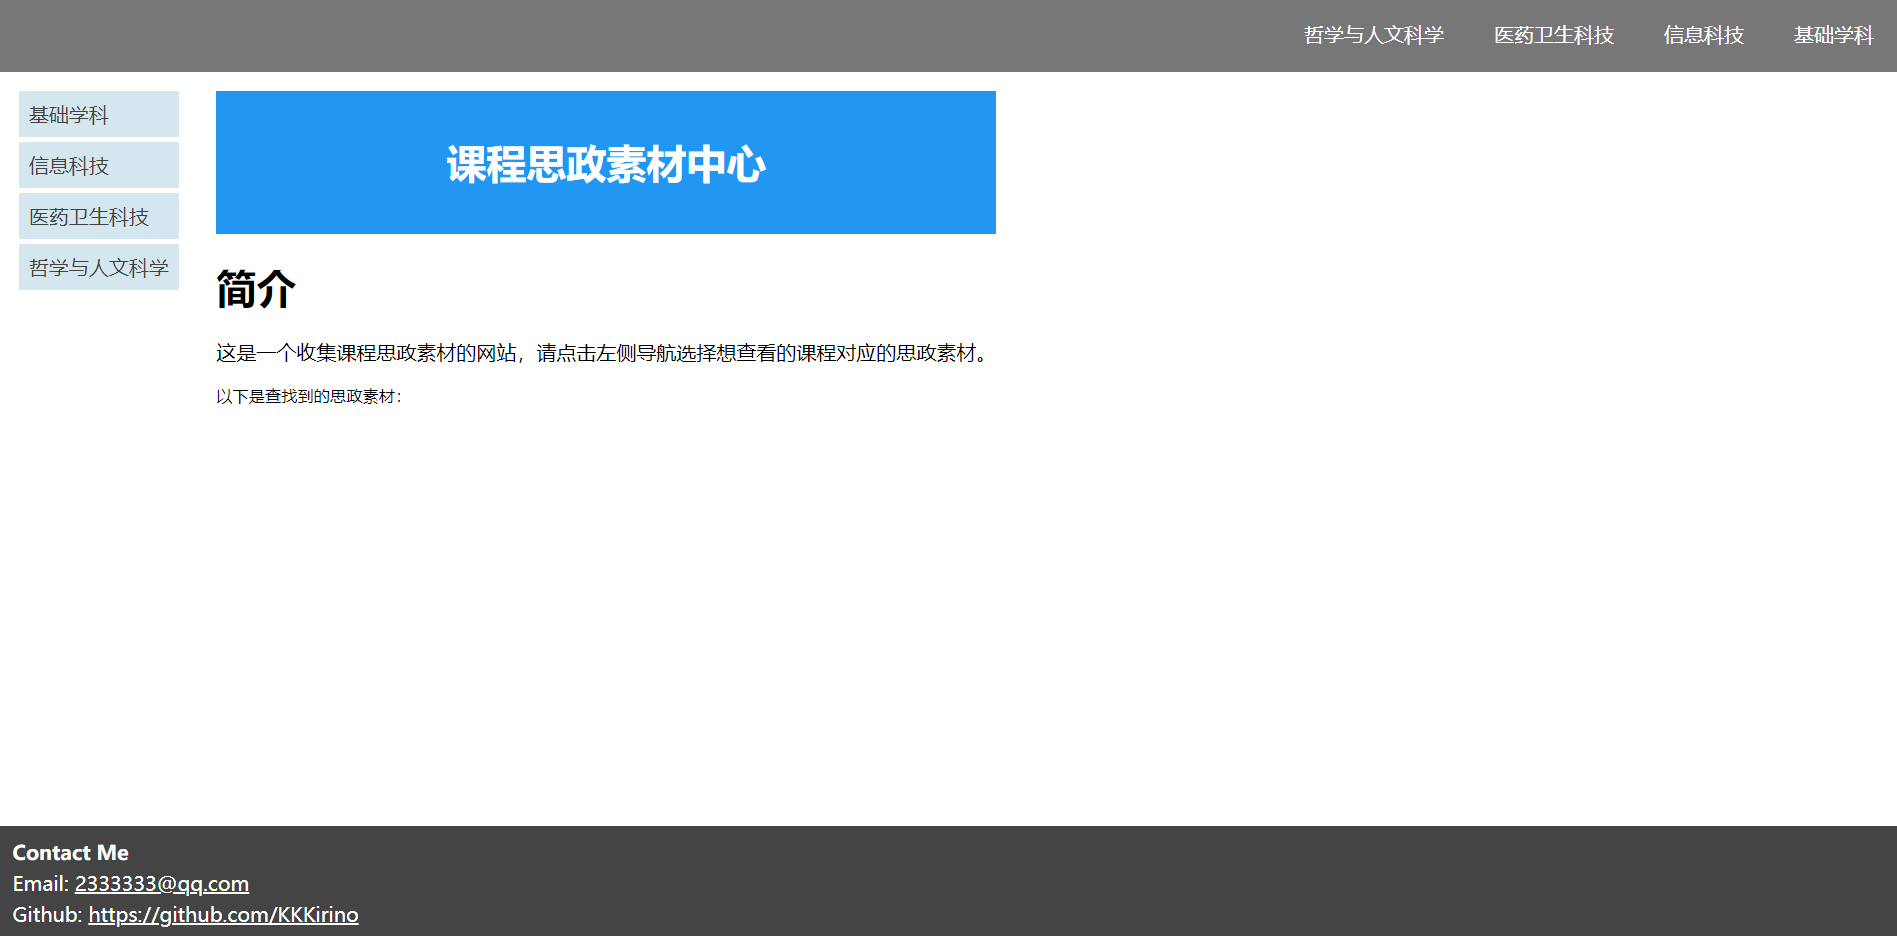
\includegraphics[width=0.9\textwidth]{home.png}
    \caption{网页主页}
    \label{fig:home}
  \end{figure*}

  点击学科,即可展示对应的思政素材,见图\ref{fig:onclick}。
  \begin{figure*}[h]
    \centering
    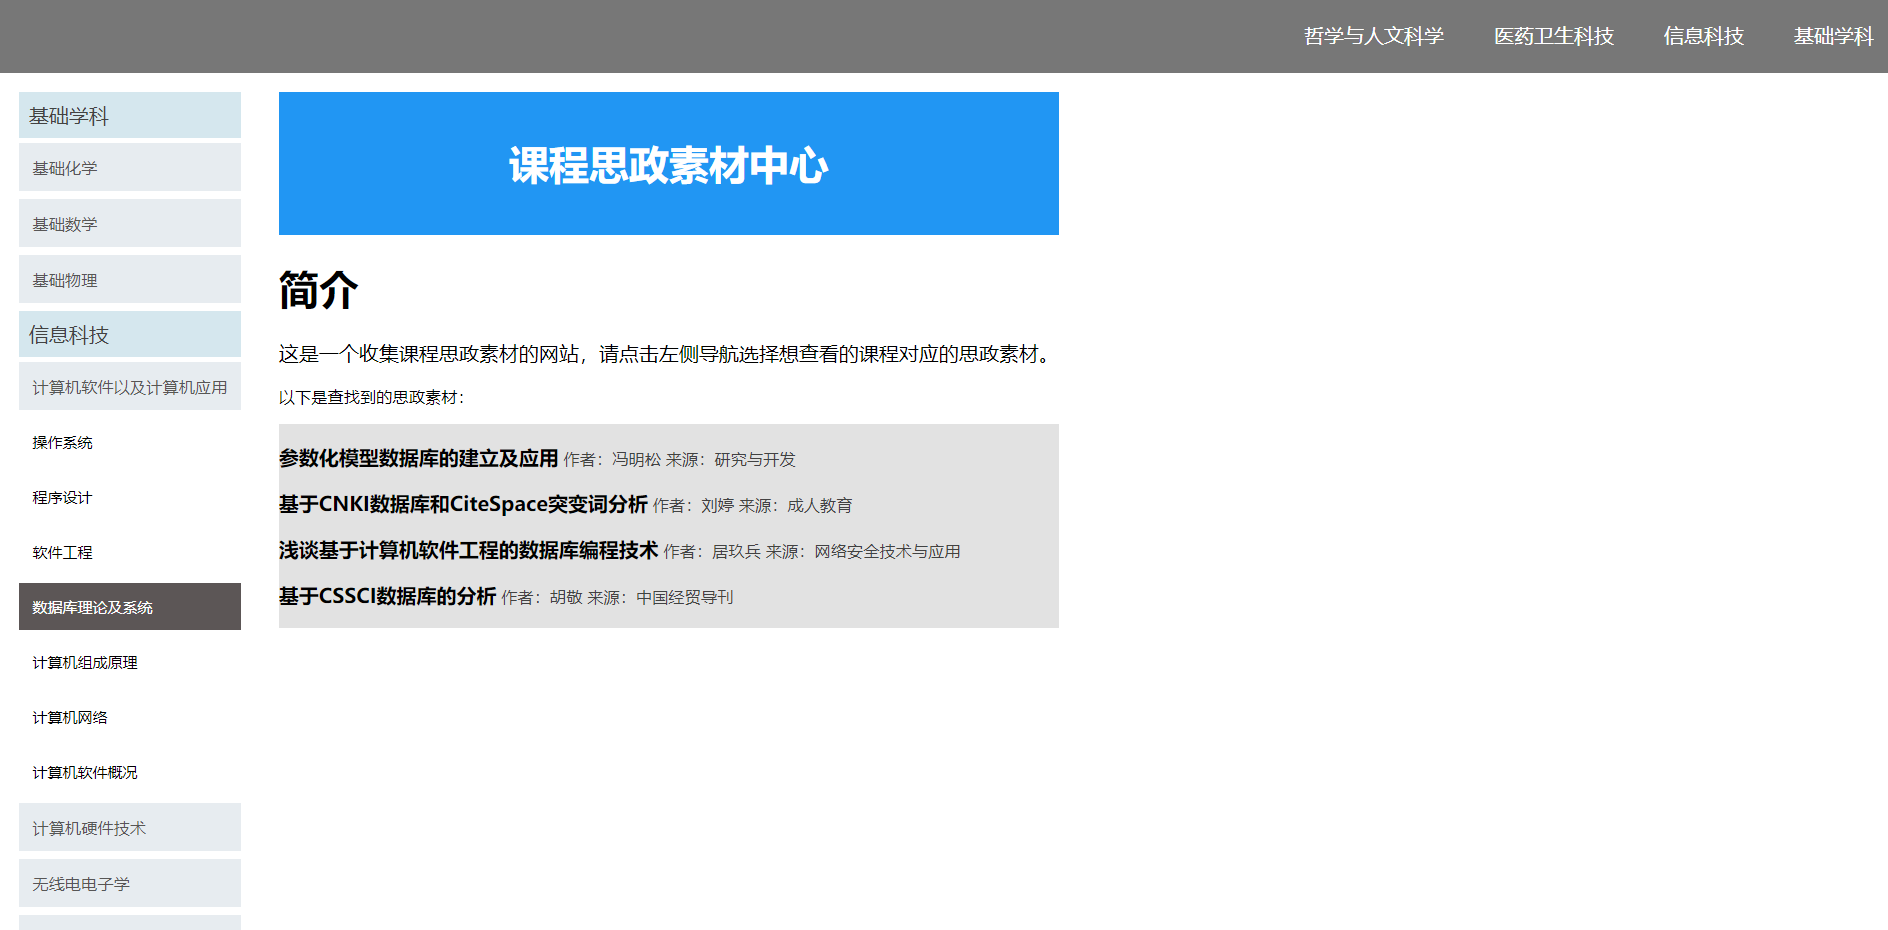
\includegraphics[width=0.9\textwidth]{onclick.png}
    \caption{展示对应的思政素材}
    \label{fig:onclick}
  \end{figure*}

  侧边栏点开,即可展示学科的树状结构见图\ref{fig:sideitem}。
  \begin{figure*}[h]
    \centering
    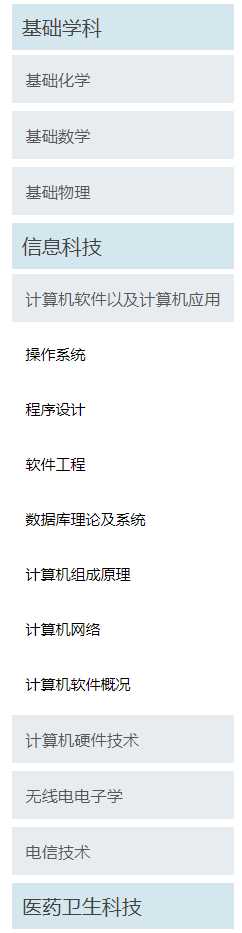
\includegraphics[width=0.2\textwidth]{sideitem.png}
    \caption{侧边栏与学科树状结构}
    \label{fig:sideitem}
  \end{figure*}


  \pagebreak

  \section{思考题}
  \pmb{Q:如何在 Power Designer 中自动生成数据库创建脚本 SQL Script?}

  点击生成的物理模型  $\rightarrow$ 上方的\verb|Database|选项 $\rightarrow$ 点击\verb|Generate DataBase|

  \pmb{Q:如何在 Power Designer 中自动生成数据库设计报告?}

  选中想要生成报告的模型 $\rightarrow$ 上方的\verb|Report|选项 $\rightarrow$ 点击\verb|Generate Report|

  \pmb{Q:如何实现批量思政资源数据的加载?}

  采用拼接\verb|BatchInsert|插入语句或者采用\verb|SqlBulkCopy|插入方案。

  \pagebreak
  \section{实验总结}
  本次实验完成了思政资源数据库创建与数据管理操作。在本次实验中,通过完成各种实验要求的操作,逐步熟练运用各种SQL语句。其次,为了完成前端界面的编写,去学习了\verb|Flack|框架的相关知识,同时也进行了前端编写的学习。虽然由于时间原因最终完成的网页不够美观,排版也可以更加完善,但是在这期间学习到了很多新的知识。

  以下是一些本次实验中可以继续完善的地方:

  \begin{itemize}
    \item 虽然在\verb|Flask|框架中利用路由,可以实现数据的增删改查操作,但是还不能在前端进行可视化的操作。后续可以继续完善登录功能,根据不同用户的权限完成不同的操作。
    \item 网站只能完成素材展示的功能,下载功能还未实现。后续会学习有关\verb|POST|请求的知识,完善网站功能。
    \item 多媒体数据的存储,目前实现的方式是在数据库中直接存放素材的地址,但是还未能在网站上完成展示。
  \end{itemize}
  
  \appendix
  % 附录代码开启行号
  \lstset{
	  numbers=left,
  }
 \pagebreak
  \section{附录:lab\_1.sql}
  \label{apd:labsql}
  \lstinputlisting[language=sql]{lab_1.txt}

  \pagebreak
  \section{附录:app.py}
  \label{apd:apppy}
  \lstinputlisting[language=Python]{app.txt}

  \pagebreak
  \section{附录:index.html}
  \label{apd:indexhtml}
  \lstinputlisting[language=HTML]{web.txt}

  \pagebreak
  \section{附录:index.js}
  \label{apd:indexjs}
  \lstinputlisting[]{index.txt}

  \pagebreak
  \section{附录:styles.css}
  \label{apd:stylescss}
  \lstinputlisting[]{css.txt}
\end{document}